\documentclass[conference]{IEEEtran}
\IEEEoverridecommandlockouts
%--------------------------------------------------------------------------------
% The preceding line is only needed to identify funding in the first footnote. If that is unneeded, please comment it out.
%--------------------------------------------------------------------------------
% Citations enabled
\usepackage{cite}
%--------------------------------------------------------------------------------
% Math package
\usepackage{amsmath,amssymb,amsfonts}
%--------------------------------------------------------------------------------
% Pseudo-code
\usepackage{algorithmic}
%--------------------------------------------------------------------------------
% Include Figures
\usepackage{graphicx}               
\usepackage{graphics} 
% \usepackage[tight,footnotesize]{subfigure}
\usepackage{caption}
\usepackage{subcaption}
%--------------------------------------------------------------------------------
% Additional text tools/colors
\usepackage{textcomp}
\usepackage{xcolor}
%--------------------------------------------------------------------------------
\begin{document}
%--------------------------------------------------------------------------------
\title{MAEG5755 Final Project - Type \#}

\author{
\IEEEauthorblockN{1\textsuperscript{st} Given Name Surname}
\IEEEauthorblockA{\textit{dept. name of organization (of Aff.)} \\
\textit{name of organization (of Aff.)}\\
City, Country \\
email address or ORCID}
\and
\IEEEauthorblockN{2\textsuperscript{nd} Given Name Surname}
\IEEEauthorblockA{\textit{dept. name of organization (of Aff.)} \\
\textit{name of organization (of Aff.)}\\
City, Country \\
email address or ORCID}
}
%--------------------------------------------------------------------------------
% Create the title page including authors
\maketitle
%--------------------------------------------------------------------------------
\begin{abstract}
The abstract is a brief summary of the whole paper. It should include brief descriptions of the six main sections of the paper: introduction or background; outstanding problems or related works; contribution; methodology; experiments and results; discussion. Each section will be explained briefly below.
\end{abstract}
%--------------------------------------------------------------------------------
\section{Introduction}
%--------------------------------------------------------------------------------
The introduction like the abstract will introduce the 6 core ideas of this paper:
\begin{itemize}
    \item Background: Introduce the general area of research: dexterous manipulation; automation; grasping. Include a diagram that helps the reader quickly connect the text with the visual representation.
    \item Problems: talk about advances that have taken place with ROS, motion planning, but also existing limitations.
    \item Contribution: in this case explain what you achieved with your project
    \item Methodology: give a brief summary of key ideas in your methodology. The use of modularized systems via ROS to achieve autonomous picking.
    \item Results: summarize quantitative or qualitative results. 
    \item Discussion: discuss the key significance of your project. What should the reader remember as the key thing. 
\end{itemize}

The length is not strict. I would expect 4 to 6 pages would be adequate. Do not write just to occupy space. Make your writing meaningful.
%--------------------------------------------------------------------------------
\section{Related Works}
%--------------------------------------------------------------------------------
The ultimate purpose of the 'Related Works' section is to point out existing weaknesses of existing research. To do that, however,  you must also explain how the research has developed. With each paper, you show how authors contributed an improvement, how their ideas work, but at the end, you will point out the existing weaknesses. 

If you are doing a simple project, look at our textbook and identify cited papers for the main parts of our course: SE(3) definition work; trajectories; forward kinematics and DH parameters; inverse kinematics and analytical or numerical methodology; PID controller, poin cloud surface detection; ROS; etc. 
%--------------------------------------------------------------------------------
\section{Methodology}
Present a detailed, logically-ordered, presentation of methods used in your work. Include any key mathematical equations, pseudo-code, etc. 

First paragraph should be an overview of the section along with a system-flow diagram that summarizes your work in a key way. Use subsections and sub subsections to arrange the code. If you are doing a ROS based project think about ex planing each of the subsystems running in your experiment and explaining each of them. 
%--------------------------------------------------------------------------------
\subsection{Subsection Example}
%--------------------------------------------------------------------------------
Here is the example of an equation
%--------------------------------------------------------------------------------
\begin{equation}
   \mathbf{z}_{v_i}^{'} = \sum_{v_j \in N_i} \alpha_{ij}^\prime \mathbf{w}_{v_j}. 
\end{equation}
%--------------------------------------------------------------------------------
And an example of an equation array:
%--------------------------------------------------------------------------------
\begin{eqnarray}
   \mathbf{a}_{v_i}=f_{aggregate}  
   \left(  
      \left\{ 
         \mathbf{h}_{v_j} : v_j \in \NC_i  
      \right\}
   \right) \\
    \tilde{\mathbf{h}}_{v_i} = f_{update}
    \left( 
      \mathbf{h}_{v_i},\mathbf{a}_{v_i}
    \right).
\end{eqnarray}
%--------------------------------------------------------------------------------
\section{Experiments and Results}\label{sec:experiments}
%--------------------------------------------------------------------------------
Start with an overview of the two sections.
%--------------------------------------------------------------------------------
\subsection{Experiments}\label{sec:experiments}
%--------------------------------------------------------------------------------
In this section, give a detailed explanation of the experimental setup; such that if there was a person reading your paper, they could run the experiments from your explanation. Typically you would describe the following:
\begin{itemize}
    \item Testbed: robot, sensors, computers.
    \item Software: OS, ROS distro, packages used for 
    \item Task: environments, parts, sequence of the task.
\end{itemize}
%--------------------------------------------------------------------------------
\subsection{Results}
%--------------------------------------------------------------------------------
Result sections should provide quantitative and qualitative results of all experiments conducted along with analysis. If you do not have quantitative data to present and analyze, you can include a set of figs that show the progression of your experiment and you can describe how successfully the robot completed each step. Here is an example below:
%-------------------------------------
\begin{figure*}[htb]
     \centering
     \begin{subfigure}{0.4\textwidth}
         \centering
         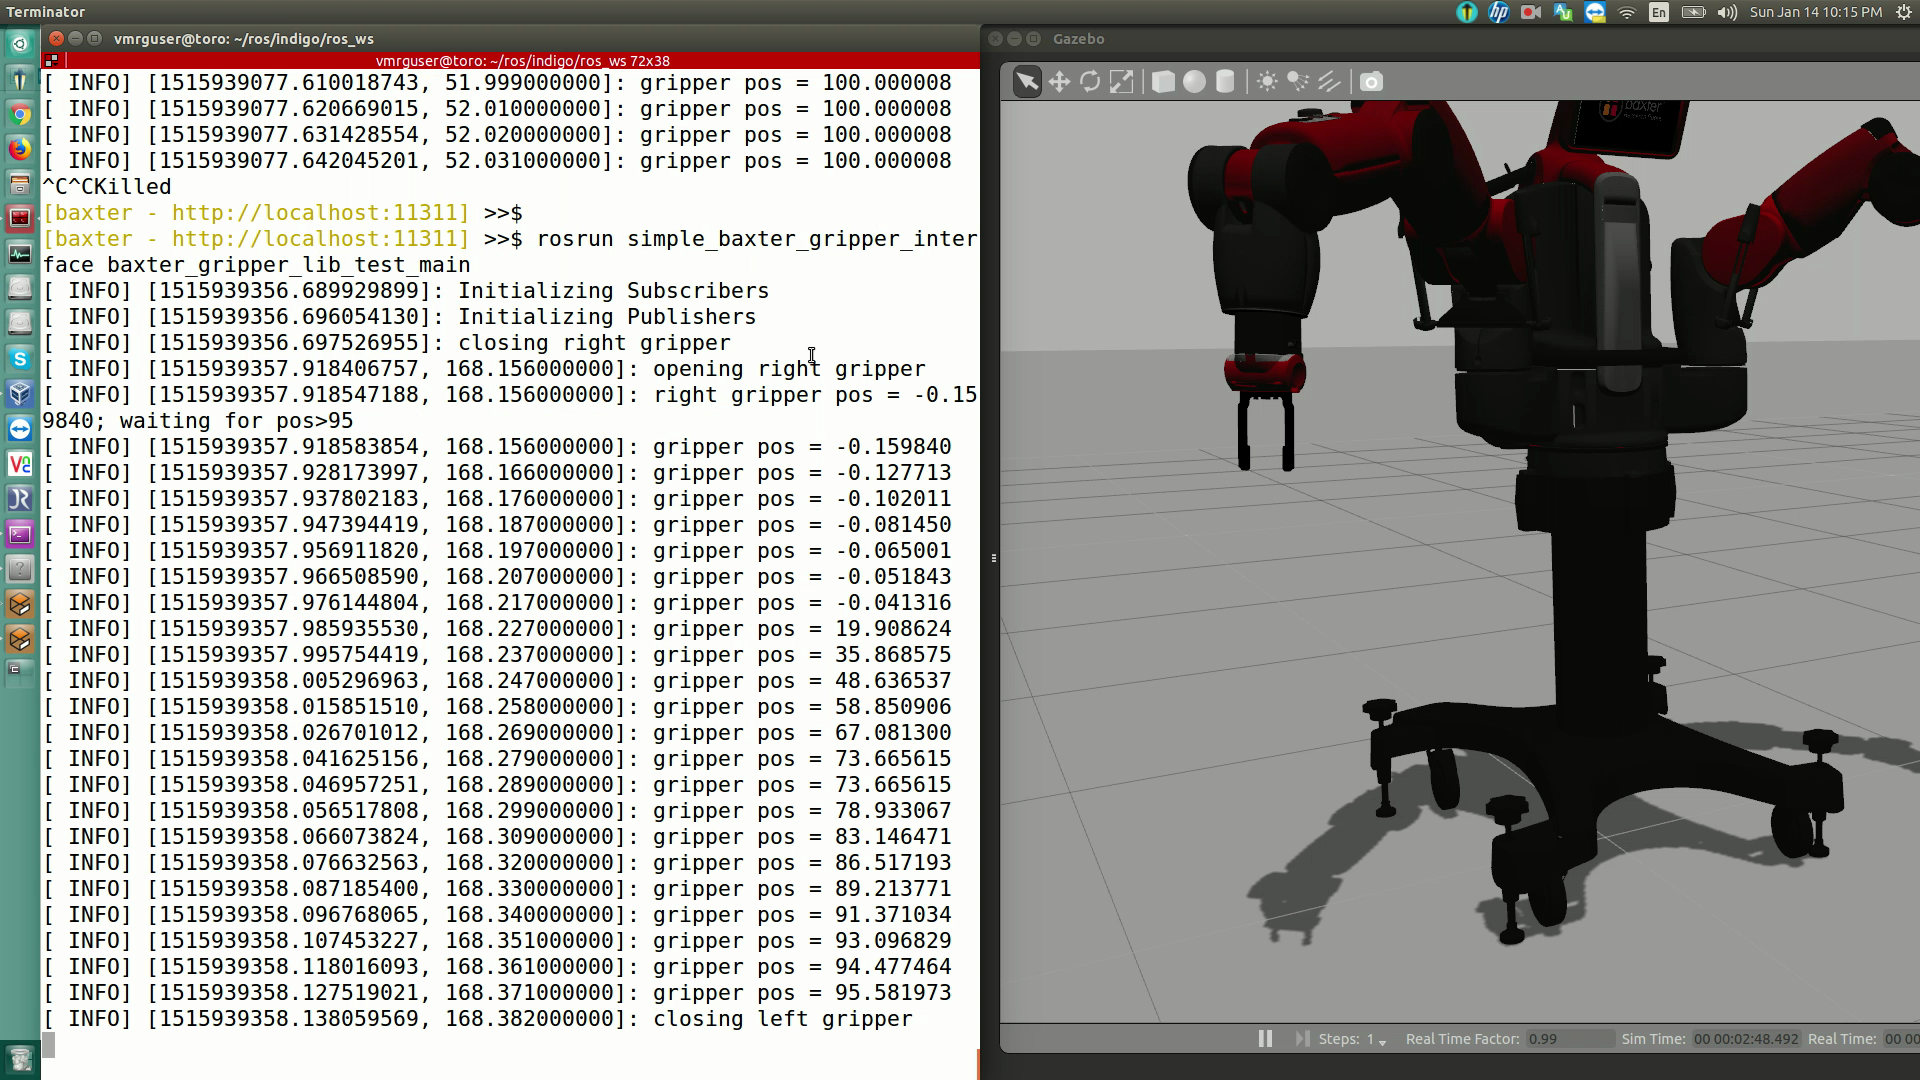
\includegraphics[width=\textwidth]{pics/baxter.png}
         \caption{subfig1.}
         \label{fig:rob_traj_reflection}
     \end{subfigure}
     \hspace{0.5cm}
     \begin{subfigure}{0.4\textwidth}
         \centering
         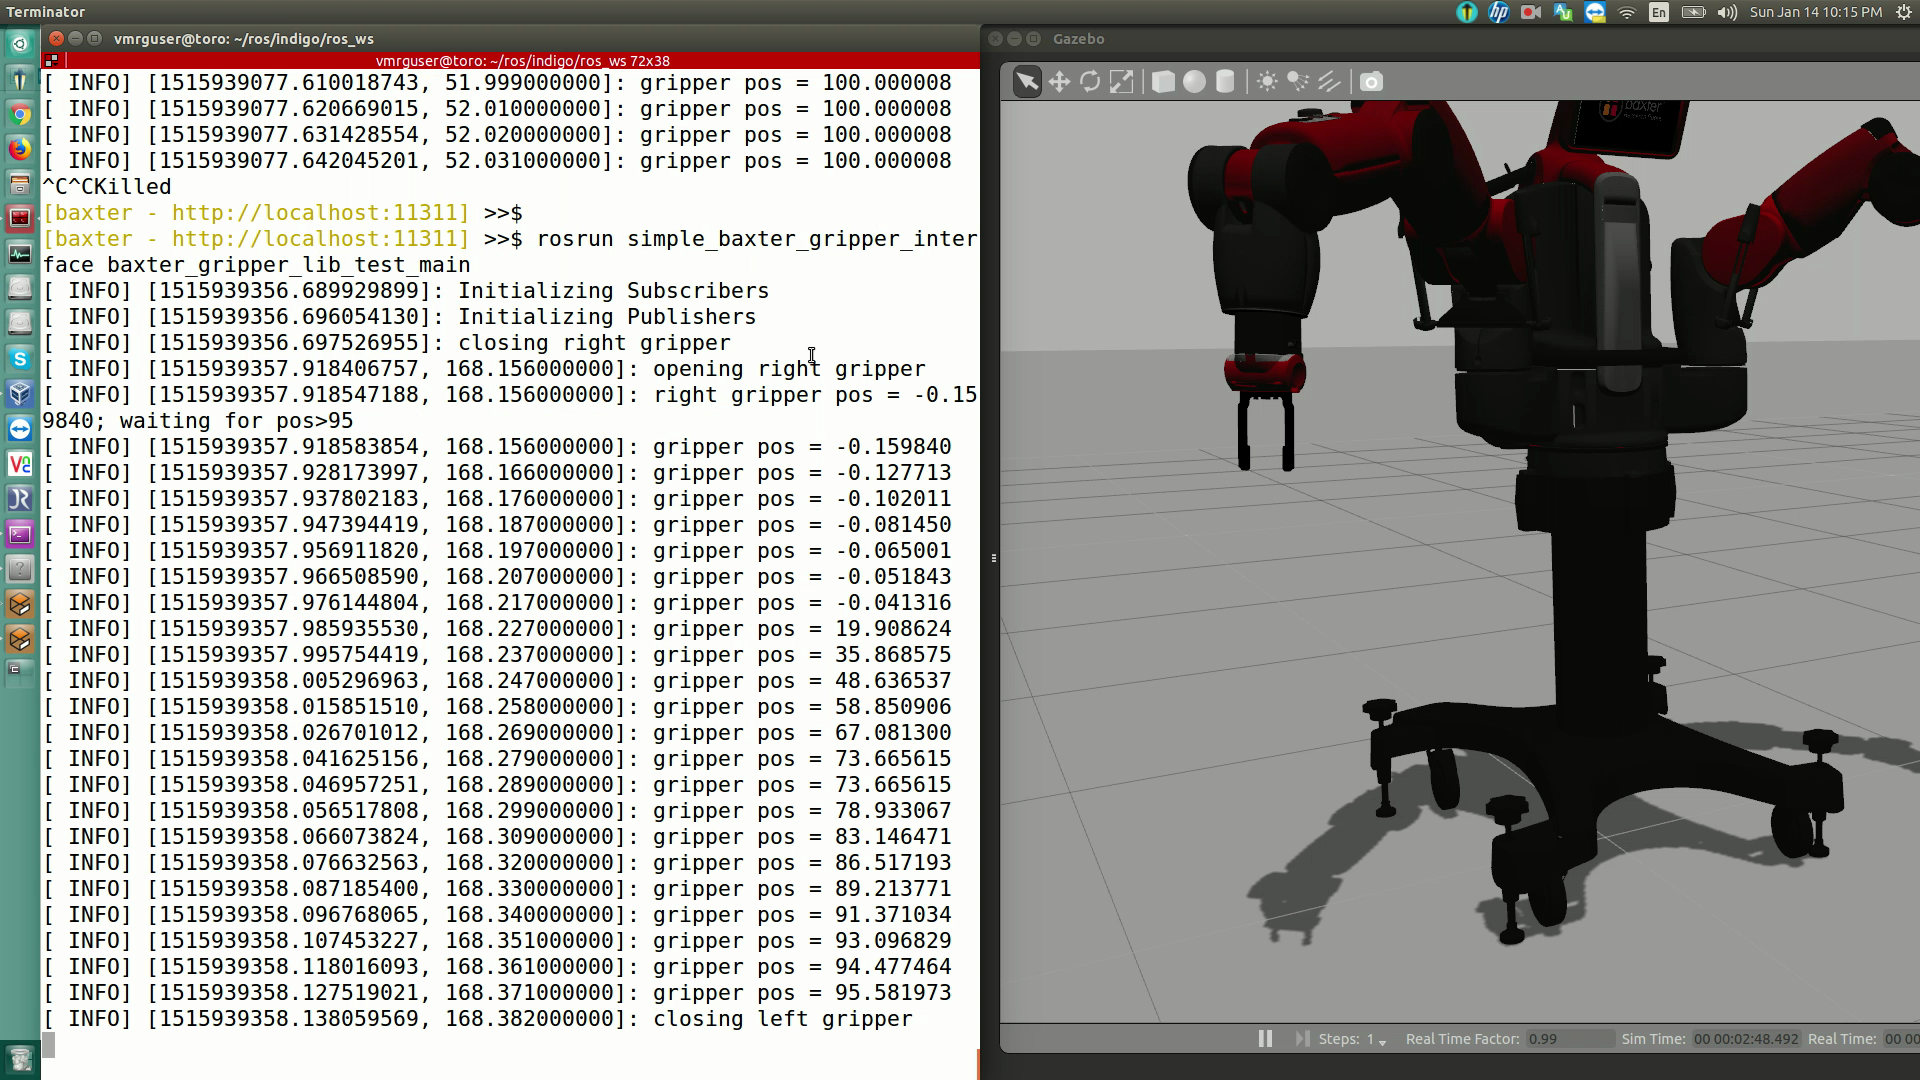
\includegraphics[width=\textwidth]{pics/baxter.png}
         \caption{subfig2.}
         \label{fig:trajectory_reflection}
     \end{subfigure}
     \caption{Temporal sequence of experiment. Make all figure captions present complete detail of what is shown. We say captions must stand-alone. }
     \label{fig:iter}
\end{figure*}
%-------------------------------------
%--------------------------------------------------------------------------------
\section{Discussion}
%--------------------------------------------------------------------------------
In a typical Discussion section for a research paper you would discuss the following three things:\\
%--------------------------------------------------------------------------------
\begin{itemize}
    \item State that your results confirm your contribution
    \item Strengths: discuss the strengths of your paper based on evidence and compared to other works in the literature
    \item Weaknesses: discuss shortcomings and explanations or reasons in  your work, and if possible how they can be addressed.
\end{itemize}
%--------------------------------------------------------------------------------
In this project, however, you cannot compare strengths or weakness with related works so instead do as follows:
%--------------------------------------------------------------------------------
\begin{itemize}
    \item Discuss the most critical lessons that you learned in realizing this project. Particularly associated with theory (e.g. inverse kinematic computation for Baxter; algorithms for Cartesian/motion planning; pose estimation for target objects via surface identification); the way  or programming: ROS middleware decentralized graph; the hierarchical structure used to modularize and generalize the manipulation system;  
    \item Existing weaknesses of the current system. The discussion should be focused on specific aspects. Explain why they are a weaknesses and present alternative proposals. 
\end{itemize}
 %--------------------------------------------------------------------------------
\begin{thebibliography}{00}
% Below an example of how to create a bibliography/references. 
% Note, however, there are better ways to enter bibliography using a .bib file. Bib files can also be easily created using software like zotero/mendeley/jabref/etc.
% Check the overleaf documentation if you prefer to do that it that way. 
%--------------------------------------------------------------------------------
\bibitem{b1} G. Eason, B. Noble, and I. N. Sneddon, ``On certain integrals of Lipschitz-Hankel type involving products of Bessel functions,'' Phil. Trans. Roy. Soc. London, vol. A247, pp. 529--551, April 1955.
\bibitem{b2} J. Clerk Maxwell, A Treatise on Electricity and Magnetism, 3rd ed., vol. 2. Oxford: Clarendon, 1892, pp.68--73.
\bibitem{b3} I. S. Jacobs and C. P. Bean, ``Fine particles, thin films and exchange anisotropy,'' in Magnetism, vol. III, G. T. Rado and H. Suhl, Eds. New York: Academic, 1963, pp. 271--350.
\bibitem{b4} K. Elissa, ``Title of paper if known,'' unpublished.
\bibitem{b5} R. Nicole, ``Title of paper with only first word capitalized,'' J. Name Stand. Abbrev., in press.
\bibitem{b6} Y. Yorozu, M. Hirano, K. Oka, and Y. Tagawa, ``Electron spectroscopy studies on magneto-optical media and plastic substrate interface,'' IEEE Transl. J. Magn. Japan, vol. 2, pp. 740--741, August 1987 [Digests 9th Annual Conf. Magnetics Japan, p. 301, 1982].
\bibitem{b7} M. Young, The Technical Writer's Handbook. Mill Valley, CA: University Science, 1989.
\end{thebibliography}
%--------------------------------------------------------------------------------
\end{document}
%--------------------------------------------------------------------------------